\chapter{Theory and Scope}
In this Chapter the scope for the study will be set.  We dig into visual perspectives and defined by a continuum from ego-centric to exo-centric. Movements will be classified and investigated how to measure movements. Eventually, a definition of mixed reality is provided. If not other indicated, adopted from the book Motor Learning and Skills\cite{Schmidt2011}.

\section{Visual Perspectives}
Wang and Milgram \cite{Wang2001} describe the perspectives on the centricity continuum see figure \ref{fig:ego-exo-cont}. On the most left hand side of the continuum the egocentric perspective is located. Egocentric means that the anchor of the viewport camera is located inside the object to control - for simplicity, this object in question is referred as avatar. On the right hand side the exocentric perspective is located. This viewport camera is a fixed camera in the scene not to be controllable. The exocentric perspective gives the user the possibility to examine the scene from a bird's-eye view. The movement or angle of the avatar has no influence on the cameras position or angle. So the main difference is the so called tether distance and the degree of freedom of the camera. Milgarm and Wang investigated on tethered cameras and define it as the distance between the eyes of the avatar and the camera which is following the avatar. This describes the middle part of the continuum. Zero-distance camera describes the egocentric perspective. The longer the tether distance the more the perspective is located on the right of the scale to the exocentric perspective. They also distinguish between dynamic and rigid tethering relationships. A dynamic tethered camera is controlled by the user in all six degree of freedoms (dof) while a rigid stands like a pole and can only be controlled in 3 dofs. Rigid tethered cameras are common in modern 3rd person computer games.
\begin{figure}
	\centering
	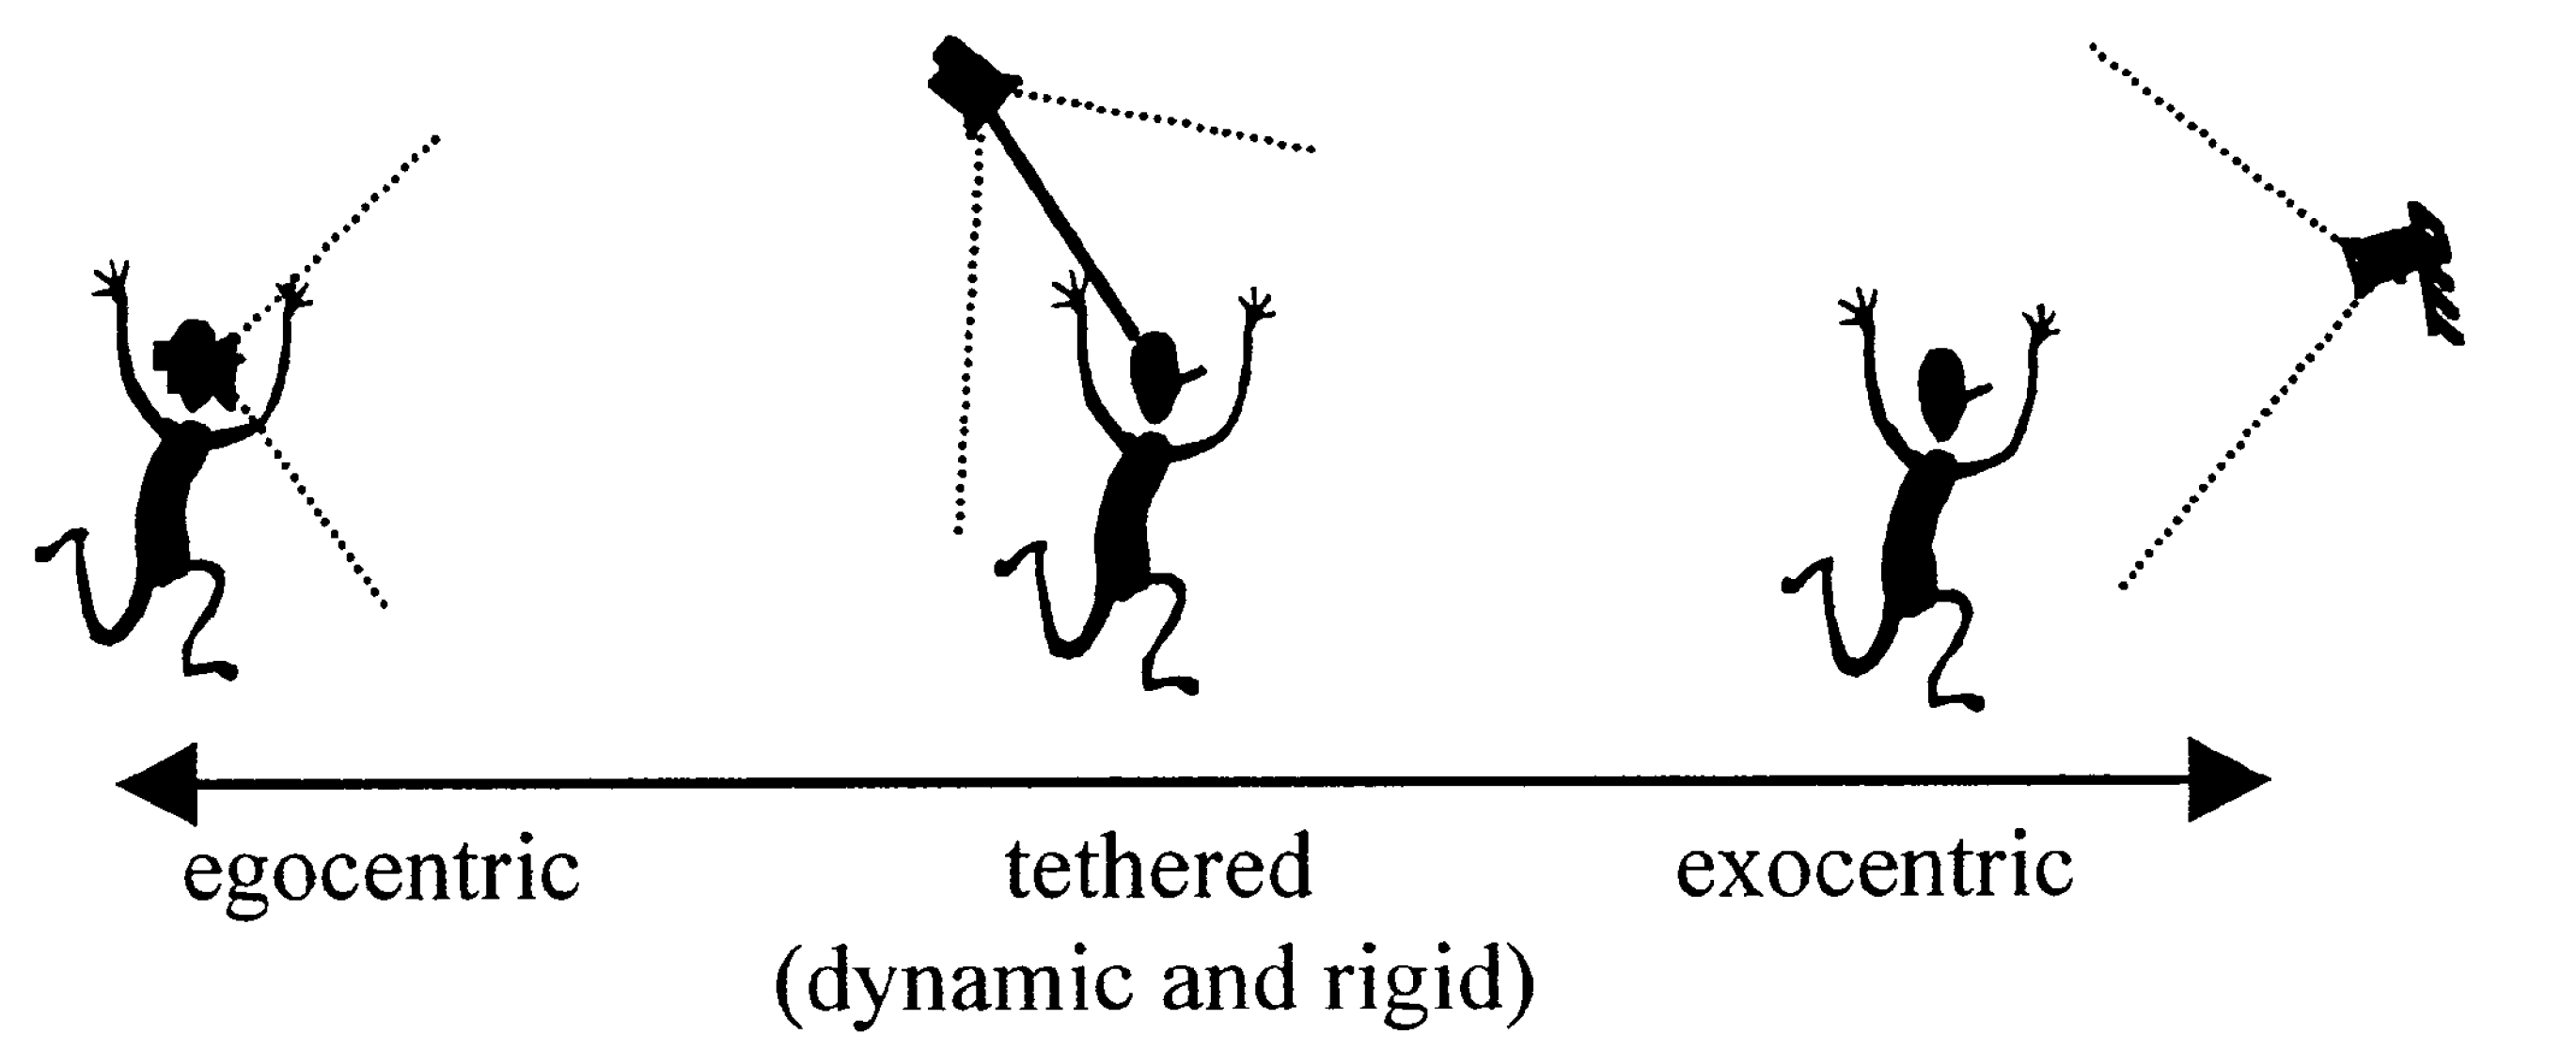
\includegraphics[width=1.0\textwidth]{img/ego_exo_continuum_bigger.PNG}
	\caption{Centricity continuum by Wang and Milgram 2001 \cite{Wang2001}}
	\label{fig:ego-exo-cont}
\end{figure}

\section{Motor Learning}
\subsection{Learning movements}
Motor learning takes place by instruction, trying, imitation or a combination of two or all three. A learner can observe another person and imitate the movement, try to accomplish a task by themself or can follow instructions. Instructions can be written, visual or verbal. Written instructions are not bound to words solely, eg. Rudolf van Laban developed a dance notation system, compare figure \ref{fig:laban}.
\begin{figure}
	\centering
	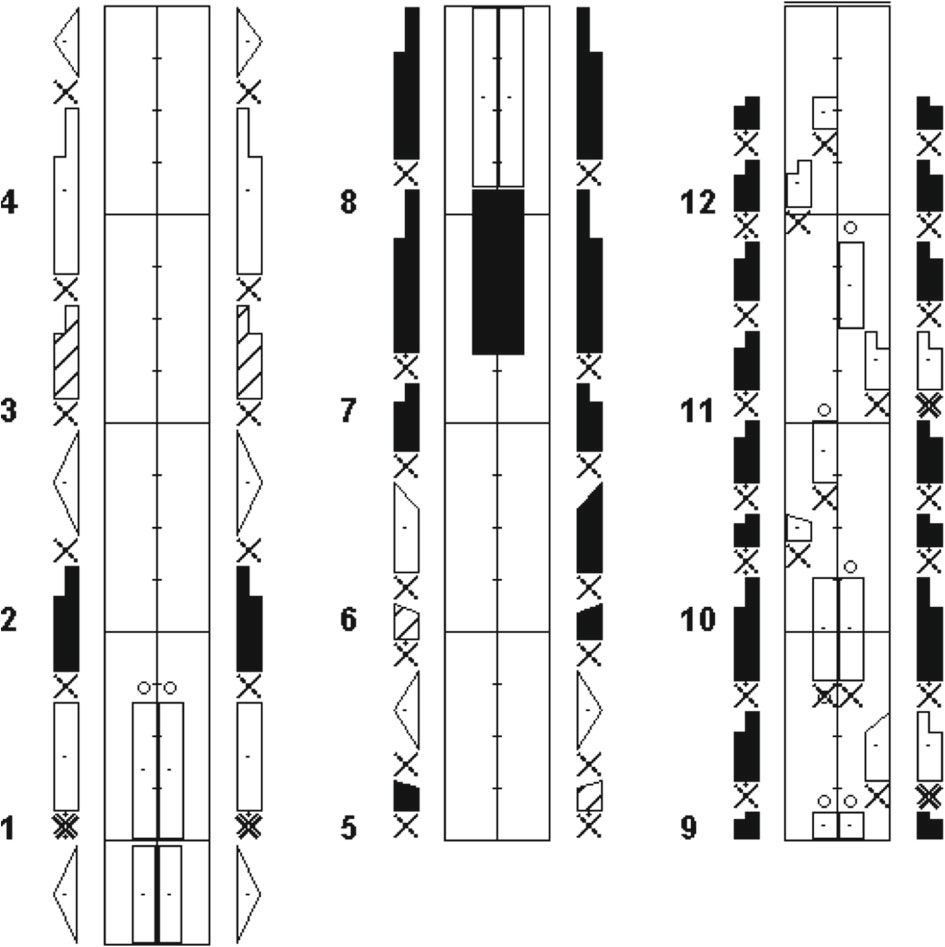
\includegraphics[width=0.5\textwidth]{img/laban.png}
	\caption{Laban notation. Generated through automatic movement interpretation by Choensawat \cite{Choensawat2015}}
	\label{fig:laban}
\end{figure}
Visual or verbal instruction include a trainer, teaching the student movements. In this case verbal and physical feedback also plays a role in the learning process. The process of motor learning is divided in three parts. Once a student starts learning using a technique, the student starts in the \textit{cognitive} state. In this stage the students tries to figure out what is to be done to achieve the task. For this high cognitive activity is required, strategies are evaluated. The performance gains dramatically and is larger than in any other stage, but also inconsistent. The use of instructions and other training techniques are most effective. The next stage is the \textit{associative}. It begins when the student had determined the most effective way of doing the task. Performance increases more gradually but becomes more consistent. In the last \textit{autonomous} stage, the performer gains proficiency and other tasks are less likely to interfere. \underline{Since the use of training techniques and the high performance gain in the \textit{cognitive} state and the use of training methods are most effective, tasks in this stage are best suited for the study.}\\
%maybe sth about time and money

\subsection{Movement classification}
Movements can be classified. There are two common classification schemas. The first one is based on the particular movements performed and are divided into \textit{discrete}, \textit{continuous} and \textit{serial movements}, compare figure \ref{fig:movements_cont}. The second one is based on perceptual attributes of the task and are divided into \textit{open} and \textit{closed skills}, compare figure \ref{fig:skills_cont}. Both classification representing a continuum.

\subsubsection{Discrete, Continuous and Serial Movements}
\begin{figure}
	\centering
	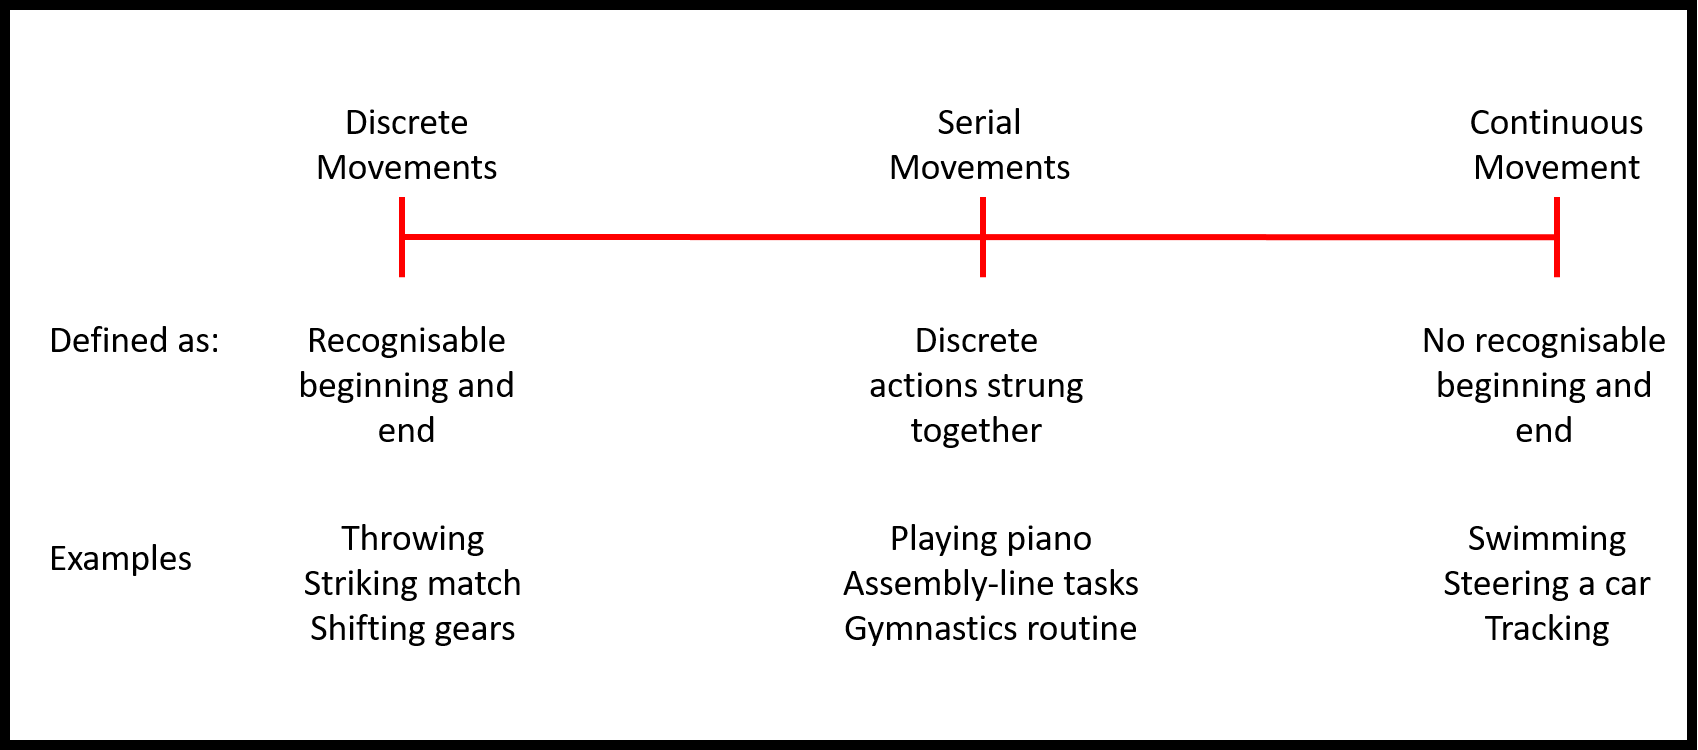
\includegraphics[width=1.0\textwidth]{img/movement_classification.png}
	\caption{Continuum of movements \cite{Schmidt2011}.}
	\label{fig:movements_cont}
\end{figure}
\textit{\textbf{Discrete movements}} are located on the one end of the continuum. These are movements with a recognisable beginning and end. The end of a discrete movement is defined by the task itself and can be very rapid like blinking or longer like making the signing. Examples are kicking a ball, shifting gears in a car or striking a match\\
\textit{\textbf{Continuous movements}} are located on the other end of the continuum. These movements don't have a recognisable start and end, with behaviour continuing till the movement arbitrarily stopped. Continuous tasks tend to be longer than discrete tasks. Examples are swimming, running or steering a car.\\
\textit{\textbf{Serial movements}} are located in the middle part of the continuum. Following the nature of a continuum these movements are neither discrete nor continuous. They can consist of smaller movements tied together. Furthermore, discrete movements can be rather long but are not stopped arbitrarily. Serial tasks can be seen as many discrete tasks strung together and the order (and sometimes timing) is important. Examples are starting a car or preparing and lighting a wood fireplace.\\
The nature of \textit{Continuous movements} having no recognizable beginning and end makes it hard to describe a distinctive task for a study design while \textit{discrete movements} are to short for a proper task, \textit{serial movements} are choose for the study task.\\
\textit{Discrete movements} are to short for a proper evaluation. Because of the nature of having no recognisable beginning and end \textit{Continuous movements} also seems not be suitable as a task in a study. Furthermore, in Chapter 3 we will see that most researchers use \textit{serial movements} as study task. \underline{Because of this, scope is set for serial movements as study task.}

\subsubsection{Open and Closed Skills}
\textit{\textbf{Open skills:}} The environment is constantly, unpredictably changing, so the performer cannot plan his activity effectively in advance. Own movements depend on the environment. For example, if a ice hockey player shoots a shot in ice hockey, his own movement is dependent on the movement of the keeper. Another example is  driving on a free way. The driver needs to adjust his own driving dependent on the behaviour of the other cars. Success in open skills is largely determined by the extend to which a individual can adapt the planned motor behaviour to the changing environment.\\
\textit{\textbf{Closed skills:}} The environment is predictable, mainly because it is stable. This means that the performer can plan his activity in advance. Examples are bowling, archery or singing. To evaluate only the motor learning and not environmental influences the study is conducted in a controlled environment in a laboratory. Thus only \textit{closed skills} are taken into consideration.\\
This work aims to evaluate the influence of the perspective on learning, not how well students can react to unforeseen changes in the environment. \ul{Though, the scope is set to \textit{closed skills.}}

\begin{figure}
	\centering
	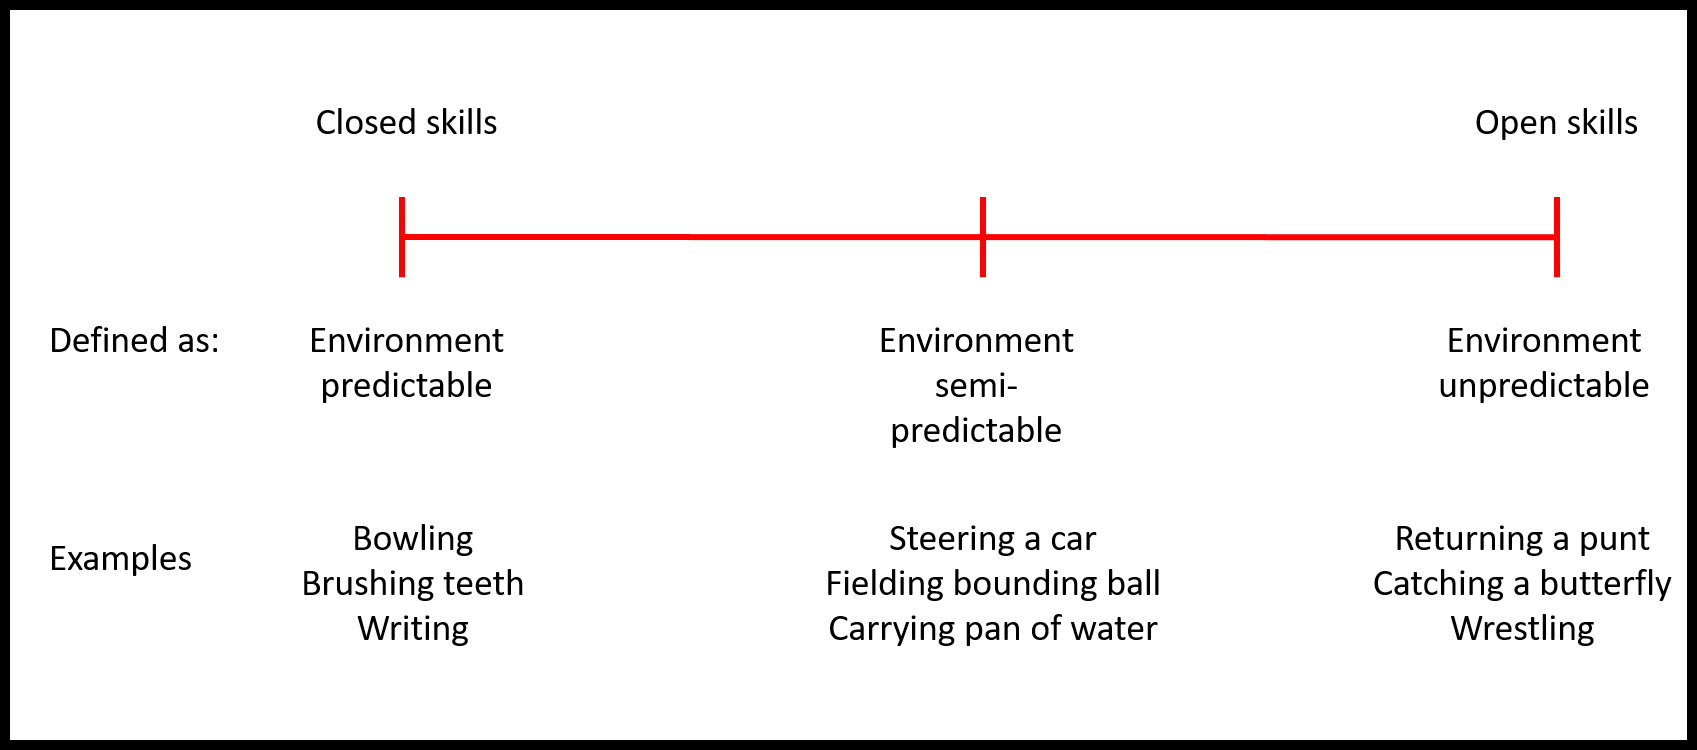
\includegraphics[width=1.0\textwidth]{img/movement_classification2.png}
	\caption{Continuum of skills \cite{Schmidt2011}}
	\label{fig:skills_cont}
\end{figure}
%since open skills  seems to require rapid adaptions to a changing environment and closed skills require a very stable performances in a predictable environment questions are raised about the method of training, do different individuals perform better in in one of these skill classes. to overcome these question the focus of this seminar is on discrete movement tasks and closed skills. $->$ see study \todo + citations



\begin{comment}
Kwon et al. \cite{Kwon2005} \todo 
\begin{itemize}
	\item K. Hachimura, K. Takashina, and M. Yoshimura, “Analysis and
	Evaluation of Dancing Movement Based on LMA,” Proc. IEEE Int’l
	Workshop Robots and Human Interactive Comm., pp. 294-299, 2005.
	\item M. Yoshimura, N. Mine, T. Kai, and L. Yoshimura, “Quantification	of Characteristic Features of Japanese Dance for Individuality Recognition,” Proc. IEEE Int’l Workshop Robot and Human Interactive Comm., pp. 193-199, Sept. 2001.
	\item G. Qian, F. Guo, T. Ingalls, L. Olson, J. James, and T. Rikakis, “A	Gesture-Driven Multimodal Interactive Dance System,” Proc. IEEE	Int’l Conf. Multimedia and Expo (ICME ’04), pp. 1579-1582, June	2004.
	\item D.Y. Kwon and M. Cross, “Combining Body Sensors and Visual
	Sensors for Motion Training,” Proc. ACM SIGCHI, pp. 94-101,	2005.
	\item vr dance trainer
\end{itemize}
\end{comment}


\subsection{Measuring movements}
%Welche messmethoden gibt es um bewegungen zu messen
To measure a movement and matching it to a given motion is not a trivial task. Since eg. dancing is a pure physical task, movements must be recognised, digitalised and judged. One approach is to use a analogue descriptions for dancing and translate them in the digital world. Choensawat \cite{Choensawat2015} began with Rudolph von Laban - a professional dancer. Von Laban developed a broadly used dance notation. His work lead to the \textit{Laban Movement Analysis} with which human movements could be quantized.\footnote{Brockhaus, Rudolf Laban. \hyperlink{http://www.brockhaus.de/ecs/enzy/article/laban-rudolf}{http://www.brockhaus.de/ecs/enzy/article/laban-rudolf (accessed 2018-10-25)}} There are four main components to systematically describe movements in the \textit{Laban Movement Analysis}: body, effort, shape and space. Each component can describe movements independently or combined. Hachimura et al. \cite{Hachimura2004} used the methodology  of \textit{Laban Movement Analysis} and adopted it to for digital movements.\\
Yoshimura et al. \cite{Yoshimura2006} followed a similar approach from another dance movement description theory called \textit{furi}. \textit{Furi} is also described by four so called \textit{indices}: \textit{kamae}, \textit{jyu-shin}, \textit{koshi}, \textit{uchiwa}. Yoshimura at all could map these indices to concrete markers on the body of a performer. Qian et al. \cite{Qian2005} developed a gesture recognition system for performing arts. To match the motions ten body parts were defined: head, torso, upper arms, forearms, upper legs and lower legs. For each body part the Mahalanobis distance is calculated to an ideal point. The Mahalonobis distance describes the distance between point \textit{p} and distribution \textit{D}.\\
To measure a movement, often single point during the movement measured repeatedly and then calculated a whole score. In literature, three main categories of those point measures are listed: \textit{error of a single subject}, \textit{measures of time and speed} and \textit{measures of movement magnitude}. As chapter 3 will show, \textit{error of a single object} is most commonly used, the latter two are only discussed in short. \ul{For this reason, measures for single error will be used to evaluate the movements in the study presented in Chapter 4.}
\subsubsection{Measures of Error for a Single Subject}
Measures of error for a single subject represent the degree to which the target was not achieved. A target can be to perform an act at a particular time (time stamp), move with a certain force (amount of force) or hit a spatial target (a point in spatial volume). The attribute of the target serves as the variable in question, see braces behind the examples. The error itself describes the distance - in regard to the dimension - from the target. The following list gives an insight to the most important error measures.
\begin{itemize}
	\item \textbf{\textit{Constant Error}} describes the average error between the actual accuracy and the target. Means, in average the performer missed the target by CE.
	\begin{equation}
		CE=\frac{\sum_i(x_i-T)}{n}
	\end{equation}
	\label{eq:constanterror}
	with $x_i$: score, $n$: number of values, $T$: target value.
	\item \textbf{\textit{Variable Error}} measures the inconsistency in movements. The more consistent the movements, the smaller $VE$. $VE$ does not depend on whether or not the subject was close to the target.
	\begin{equation}
		VE=\sqrt{\frac{\sum(x_i-M)^2}{n}}	
	\end{equation}
	\item \textbf{\textit{Total Variability}} describes the total variability around a target. The combination of VE and CE represents the total amount of spread about the target. It is an overall measure how successful was the subject in achieving the target.
	\begin{equation}
		E=VE^2+CE^2=\sqrt{\frac{\sum(x_i-T)^2}{n}}
	\end{equation}
	with $x_i$: score, $n$: number of values, $T$: target value.
	\item \textbf{\textit{absolute error}} is a measure of the overall accuracy in performance.
	\begin{equation}
		AE=\frac{\sum|x_i-T|}{n}
	\end{equation}
	with $x_i$: score, $n$: number of values, $T$: target value.
	\item \textbf{\textit{Absolute Constant Error}} is the absolute value of $CE$. Because of negative and positive values can cancel each other out
	\begin{equation}
		ACE = |CE|
	\end{equation}
\end{itemize}



\subsubsection{Measures of Time and Speed}
Basic to this idea is, a performer who can accomplish more in a given amount of time or who can accomplish a given amount of behaviour in less time is  more skillful. Measures here are
$\frac{time}{unit}$ or $\frac{units}{time}$.\\
The two most common examples are \textit{reaction time} (RT) and \textit{movement time} (MT). Reaction time describes the amount of time between a stimuli and the regarding start of a movement. This time span is important for two reasons. On the on hand, RT has a high validity for real-life tasks, and, on the other hand, RT measures the time taken for mental events like stimulus processing or decisinón making.\\
\textit{Movement time} is the time interval between the end of the RT phase, though the start of the response, and the completion of the movement. The sum of RT and MT is called \textit{response time}.
%\underline{reaction time} (RT): can also be a performance measure. a measure of time from the arrival of a sudden and unanticipated signal to the beginning of the response. 

\subsubsection{Measures of Movement Magnitude}
To measure a skill, the produced magnitude of a behaviour can used. Eg. the distance a discus is thrown. A famous example is the "ski simulator". Rubber bands hold a plated centred between two poles. The magnitude in this case is the the dislocation of the board from the centre by using full body movements.

\section{Mixed Reality}
\todo
Mixed reality continuum \cite{Milgram1994} and something about when AR or VR is better. \ref{fig:MRcont} \ref{fig:sh_cont}\todo 

\begin{figure}
	\centering
	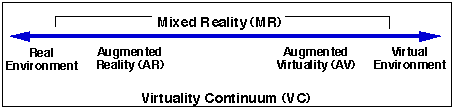
\includegraphics[width=1.0\textwidth]{img/milgram_continuum.png}
	\caption{Mixed reality continuum by Milgram et al. \cite{Milgram1994}}
	\label{fig:MRcont}
\end{figure}

\begin{figure}
	\centering
	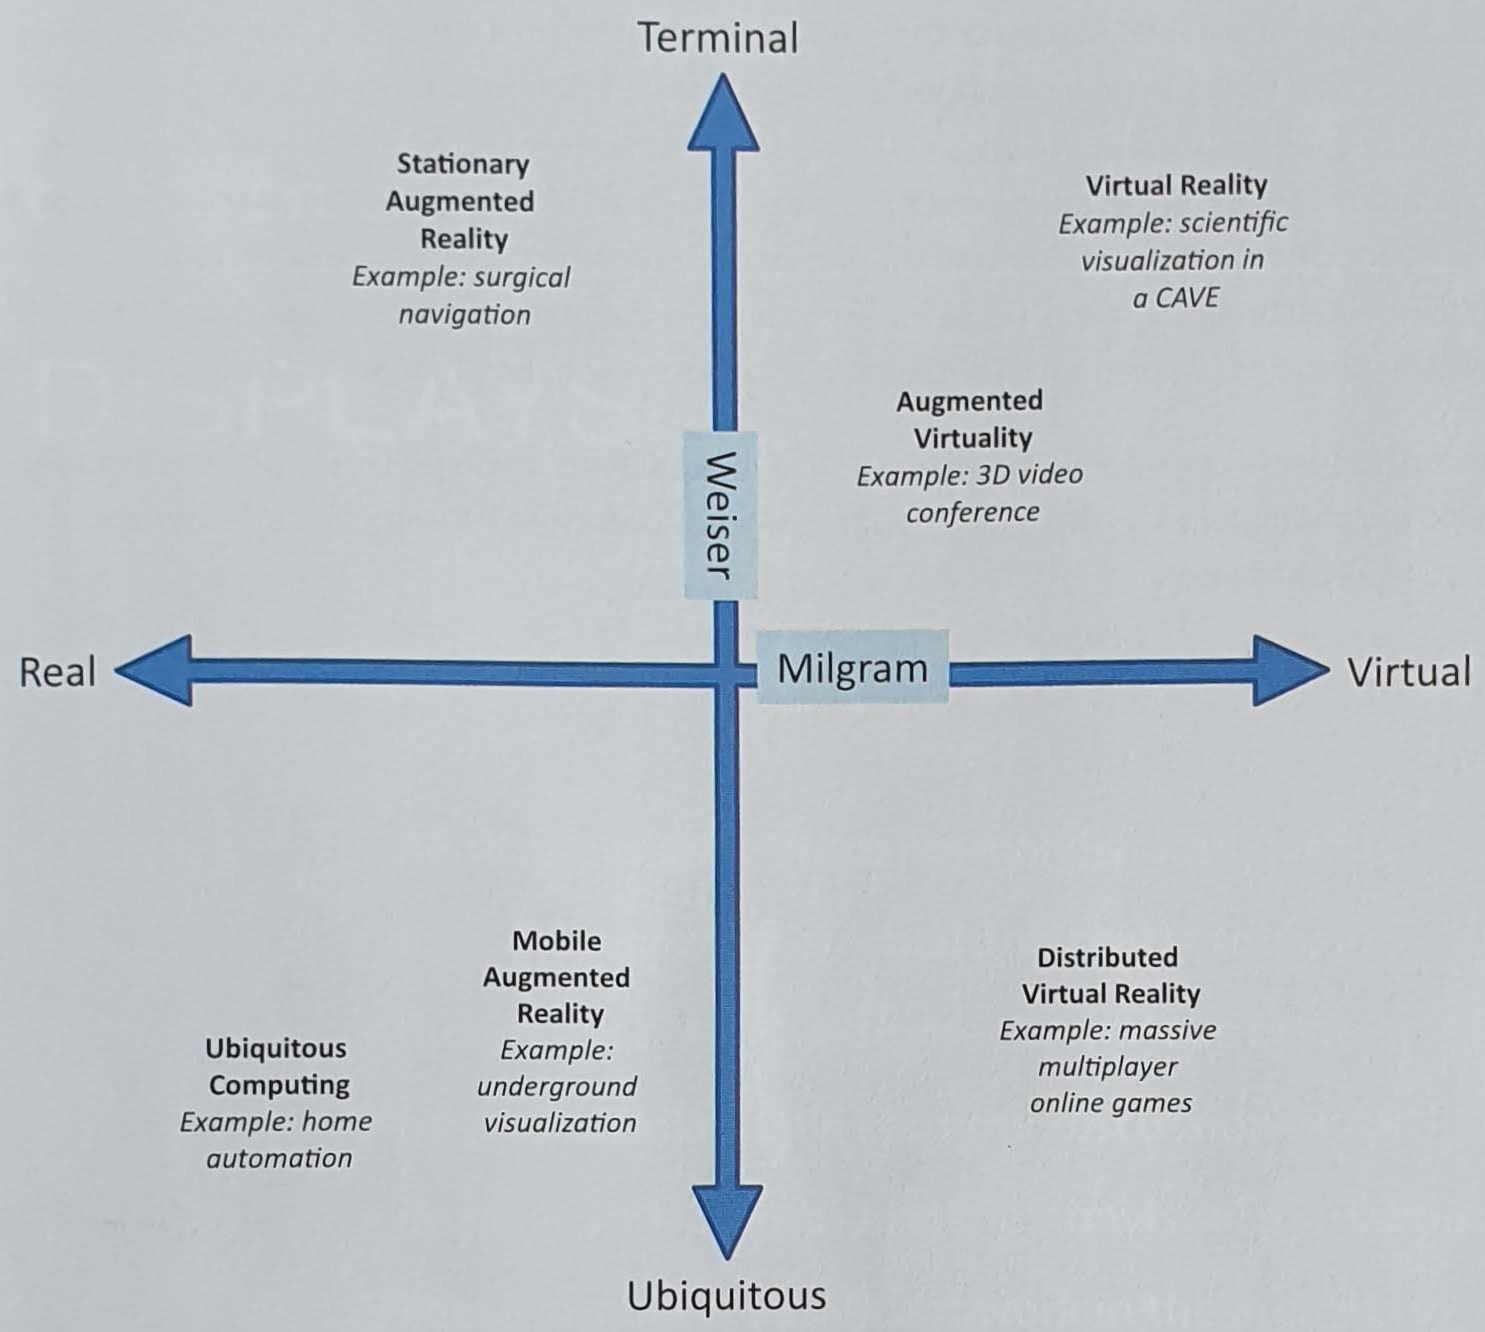
\includegraphics[width=1.0\textwidth]{img/mr_cont_sh.jpg}
	\caption{Mixed reality continuum by Schmalstieg \& Höllerer \cite{Schmalstieg}}
	\label{fig:sh_cont}
\end{figure}
\todo VR reason and compare next chapter



\section{Conclusion}
In this Chapter the scope was set. \textbf{Measures for single error} will be applied in the study to measure the movements in the study proposed in Chapter 4. The task will be a \textbf{serial task} and also only for \textbf{closed skills}.